%\documentclass[fleqn]{book}
\documentclass[11pt]{amsbook}

\usepackage[turkish]{babel}

%\usepackage{../HBSuerDemir}	% ------------------------
\usepackage{../Ceyhun}	% ------------------------
\usepackage{../amsTurkish}


\begin{document}
% ++++++++++++++++++++++++++++++++++++++
\hPage{063}
% ++++++++++++++++++++++++++++++++++++++

$ j = 4 $

\begin{center}

\begin{tabular}{ c c }  
			&	$ 1 \quad 2 \quad 3 $

			\\

    $ f_{4} = $		&	$ \left[ 1 \quad 1 \quad 1 \right] $
  
\end{tabular}

$ \overline{P}_{4} = $
\begin{tabular}{ c c }
				&       $ 1 \quad 2 \quad 3 \quad 4 $

				\\

      \begin{tabular}{c}
	1 \\ 2 \\ 3 \\ 4
      \end{tabular}		& 	$ \left[  \begin{tabular}{ c |c c c| }
						    \cline{2-4}
						    1  &  1  &  0  &  1   \\
						    1  &  0  &  0  &  0   \\
						    0  &  1  &  1  &  0   \\
						    0  &  0  &  1  &  1   \\
						    \cline{2-4}
						  \end{tabular}  \right] $
\end{tabular}

\end{center}

elde ederiz. 
$ \overline{P}_{4} $
e karşıdüşen çizge \reffig{fig:ceyhun-063-fig01} a da gösterilmiştir.
Ancak 
$ j = 5 $ 
için, 
$ A_{5} $ 
in gerçekleşmeyeceğini görürüz,

\begin{figure}[htb]
	\centering
	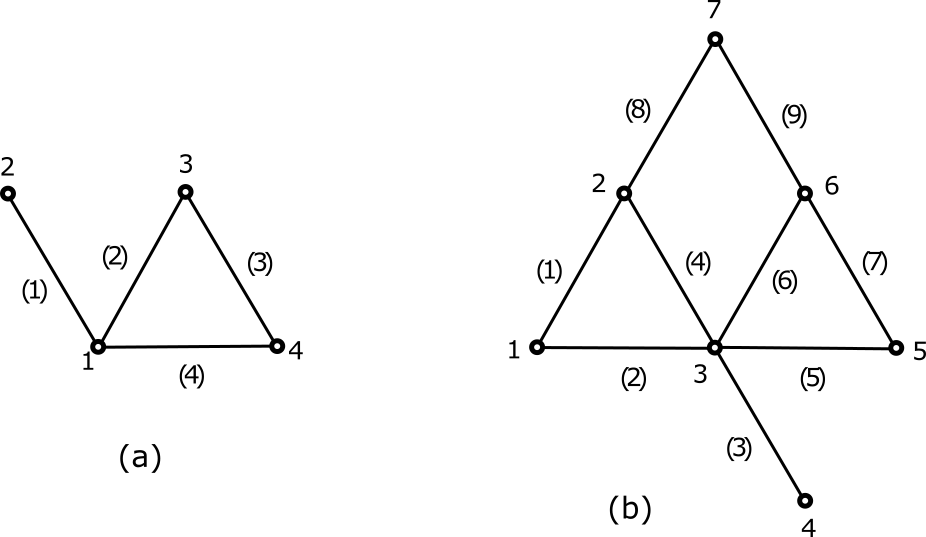
\includegraphics[width=0.9\textwidth]{images/ceyhun-063-fig01.png}
	\caption{Ayrıt matrisinin gerçekleştirimi.}
	\label{fig:ceyhun-063-fig01}
\end{figure}

\end{document}